\chapter{Additional activities during the internship}
\label{chapter:Additional activities during the internship}

\begin{introduction}
    "Always deliver more than expected." - Larry Page, co-founder of Google
\end{introduction}


\section{Additional Activities during the Internship}

As part of the internship, an additional activity involved the development of a gene panel creation tool. The purpose of the tool is to streamline the creation and management of gene panels, which are commonly used in genomic analyses.

The gene panel creator allows the user to define a panel by specifying a name and providing a list of genes. The user can paste the list of genes into the designated field, and the tool processes this input to create a gene panel. Once created, the panel becomes available within the system for further use in various analyses.

An additional feature of the tool is the generation of a \ac{bed} file containing the genomic coordinates of the genes included in the panel. This file can be downloaded directly from the tool's interface, ensuring that the user has access to the relevant genomic regions for further study. The \ac{bed} file is automatically verified to ensure that all genes are correctly recognized by the system before it is made available for download.

This gene panel creation tool was developed to improve the efficiency of handling gene panels, reducing the manual workload typically involved in their curation and preparation for analysis. The ability to automatically generate and download \ac{bed} files associated with specific gene panels has proven to be a valuable addition to the software's functionality, ultimately benefiting the genomic analysis workflows at Unilabs.

\begin{figure}[H]
    \centering
    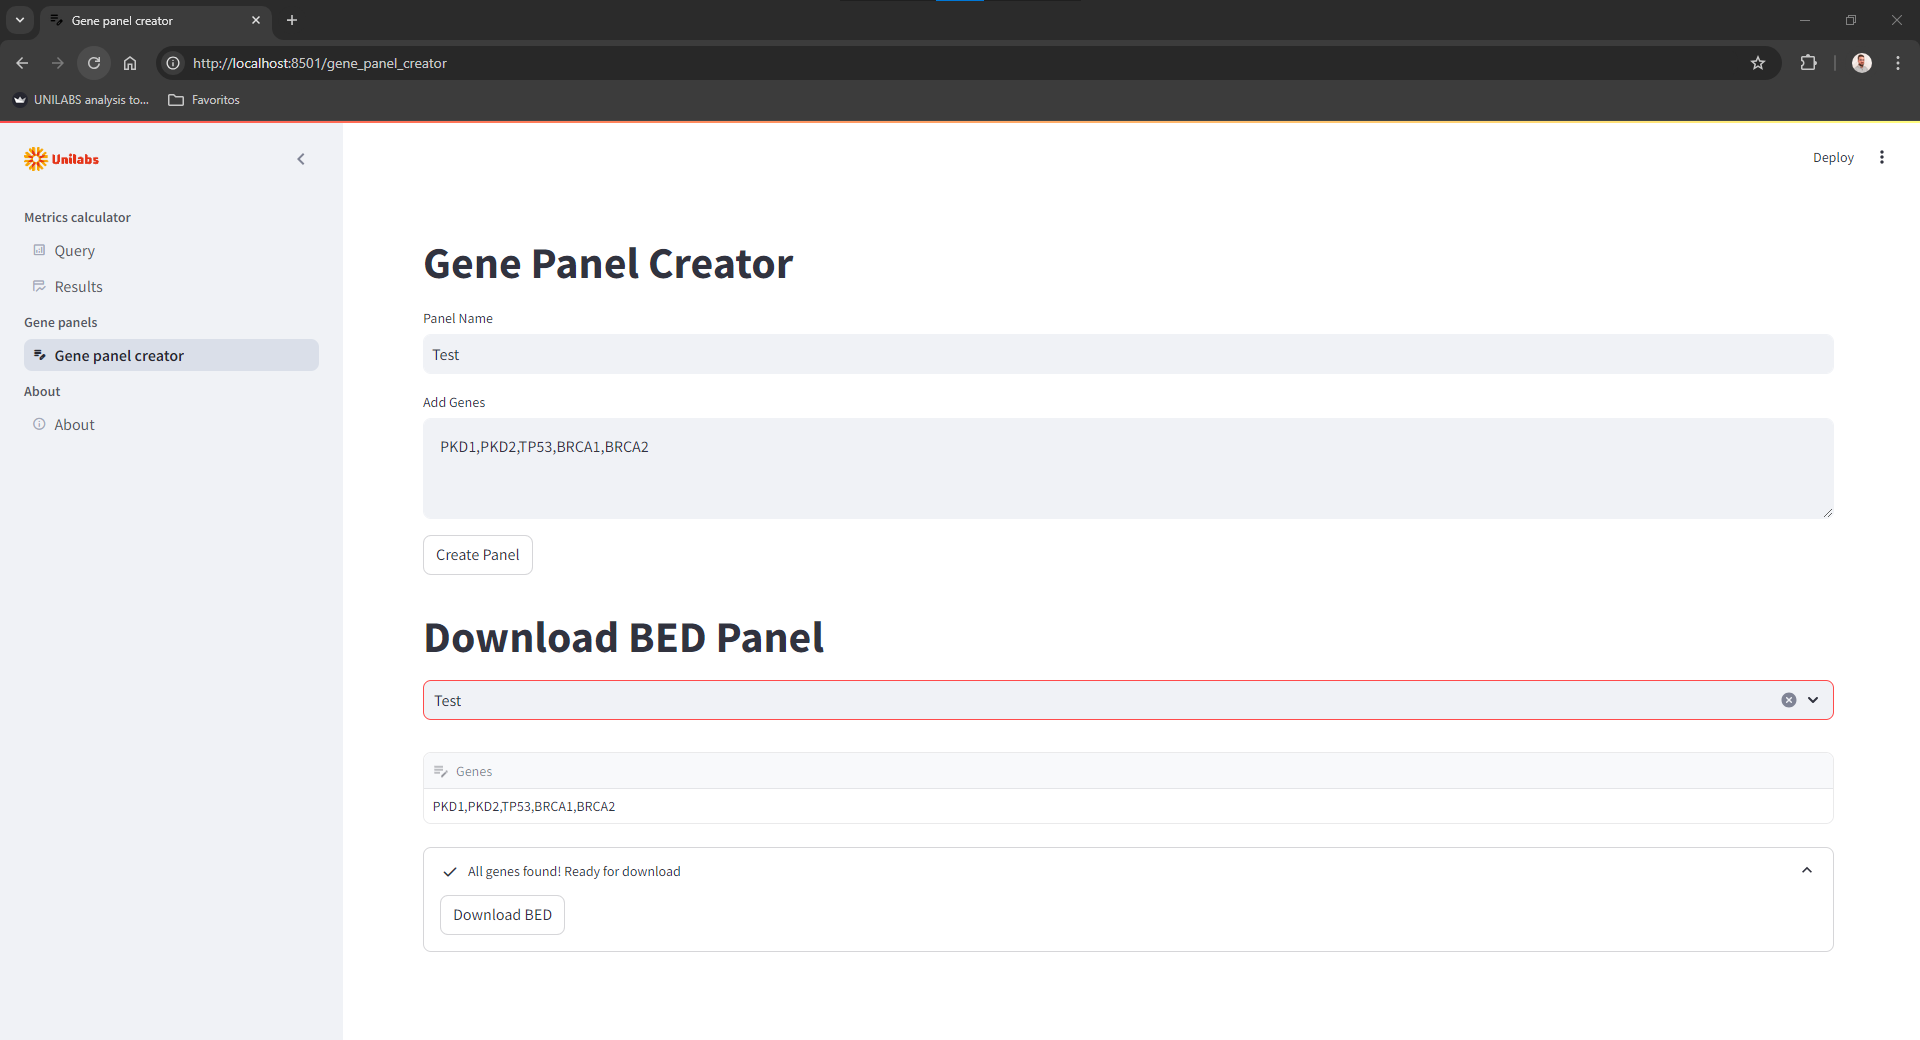
\includegraphics[width=\textwidth]{figs/v3.13.png}
    \caption{Gene Panel Creator Interface}
    \label{fig:gene_panel_creator}
\end{figure}
